% Compilar com: latexmk -lualatex case_terceiro_momento.tex
\documentclass[11pt,a4paper]{article}
\usepackage[margin=2cm]{geometry}
\usepackage{fontspec}
\usepackage{unicode-math}
\setmainfont{Latin Modern Roman}
\setmathfont{Latin Modern Math}
\usepackage[brazil]{babel}
\usepackage{booktabs,tabularx,array,graphicx,float}
\usepackage{enumitem}
\usepackage{xurl}
\usepackage[colorlinks=true,linkcolor=blue!50!black,urlcolor=blue!50!black,citecolor=blue!50!black]{hyperref}
\usepackage{xcolor}
\setlength{\parindent}{0pt}
\setlength{\parskip}{0.5em}
\newcolumntype{Y}{>{\raggedright\arraybackslash}X}
\newcommand{\arq}[1]{\texttt{\nolinkurl{#1}}}
\newcommand{\vhat}{\hat v}
\newcommand{\kthree}{\kappa_3}
\newcommand{\caixa}[2]{\par\noindent\colorbox{#1}{\parbox{\dimexpr\linewidth-2\fboxsep}{#2}}\par}

\title{Medir o terceiro momento das incertezas experimentais\\
\large Tentativa com dados reais do RHIC, validação sintética e um \emph{case} para computação quântica}
\date{25 de novembro de 2026}
\author{Proposta 4 --- \texttt{4-Fourth\_sensitivity\_test\_third\_cov\_momentum}}

\begin{document}
\maketitle
\vspace{-1.5em}

\caixa{blue!6}{\textbf{Resumo.} Na calibração bayesiana do JETSCAPE (PRC 114, 014905; 917 pontos), supor correlações nas incertezas
experimentais desloca a posterior. Na versão por setor, o deslocamento chegou a ser cerca de 3 vezes maior que na versão global.
A pergunta seguinte é se as incertezas também têm \emph{assimetria}, ou seja, terceiro momento. Para responder, fizemos um levantamento
histórico de medidas do RHIC no INSPIRE, HEPData e arXiv. Usamos as medidas repetidas do mesmo detector e as comparações entre
detectores como réplicas reais do sistemático.
\textbf{Resultado:} com os dados públicos, o \textbf{segundo momento é mensurável} (o erro de normalização é quase totalmente correlacionado
entre centralidades, $\rho_{\rm ef}=0{,}95$--$1{,}00$). O \textbf{terceiro momento não é}: a assimetria medida, $-0{,}08\pm0{,}24$, é compatível
com zero; há poucas realizações independentes ($N_{\rm ef}\approx7$); e as diferenças entre detectores só revelam a assimetria \emph{relativa}.
Em réplicas sintéticas, o Tensor PCA recupera fontes assimétricas a partir de $N\gtrsim3000$ réplicas. Esse é o problema
(\emph{spiked tensor}, $p=3$) para o qual existe um algoritmo quântico com ganho super-quadrático, o Tensor PCA quântico de Hastings.
O gargalo hoje é de \textbf{dados}, não de computação.}

% =====================================================================
\section{A pergunta}
Modelo de medida de um bloco de $n$ bins:
\[
y_{\rm exp}=\mu(\theta)+\sum_{a}\lambda_a\,\vhat_a+\varepsilon,\qquad \varepsilon\sim N(0,\mathrm{diag}\,\sigma^2_{\rm stat}),
\]
\begin{itemize}[nosep]
\item $\vhat_a$: direção da fonte sistemática $a$ (o padrão que ela imprime nos bins);
\item $\lambda_a$: amplitude, que pode ter distribuição assimétrica.
\end{itemize}
Os cumulantes de $y$ separam o que cada ordem informa:
\begin{center}
\begin{tabular}{@{}lll@{}}
\toprule
ordem & forma & o que identifica \\
\midrule
$\kappa_2=\Sigma$ & $\sum_a s_a^2\,\vhat_a\vhat_a^{\mathsf T}+\mathrm{diag}\,\sigma^2_{\rm stat}$ & só o \emph{subespaço} das fontes (há ambiguidade de rotação) \\
$\kthree$ & $\sum_a \gamma_a s_a^3\,\vhat_a^{\otimes3}$ & cada direção $\vhat_a$ e a sua assimetria $\gamma_a$ \\
\bottomrule
\end{tabular}
\end{center}
O ruído gaussiano não contribui para $\kthree$. Estimado a partir de $N$ réplicas, $\hat\kappa_3=\beta\,x^{\otimes3}+G$, com $\beta\propto\gamma\sqrt N$.
Isso é um \textbf{spiked tensor de ordem 3}.

Degraus do estudo (\arq{MAPA.tex}):
\begin{enumerate}[nosep]
\item[0.] JETSCAPE: só variâncias;
\item[1.] \emph{supor} correlações (CS/RBF, global e setor). Feito: as propostas 1 e 2;
\item[2.] \emph{aprender} o 2º e o 3º momento com dados reais. \textbf{Este documento};
\item[3.] aplicar as fontes aprendidas na calibração (nuisances $\lambda_a$);
\item[4.] escalar com Tensor PCA, clássico ou quântico.
\end{enumerate}

% =====================================================================
\section{Onde procurar réplicas reais}
O Tensor PCA precisa de muitas realizações independentes do mesmo sistemático. O STAR, o PHENIX e o PHOBOS não publicam variações
sistemáticas, só barras de erro. Procuramos duas fontes substitutas (levantamento de 17/11/2026, via INSPIRE API, HEPData e fontes \LaTeX{} do arXiv).

\subsection{\texorpdfstring{(a) O mesmo detector, medindo de novo (\arq{replicas_survey.md})}{(a) O mesmo detector, medindo de novo}}
Para as 10 medidas de referência da calibração, contamos os \emph{datasets} (runs) independentes com o mesmo observável e aceitação.
\begin{center}\small
\begin{tabularx}{\linewidth}{@{}Y c l@{}}
\toprule
medida da calibração & $N_{\rm indep}$ & observação \\
\midrule
PHOBOS $dN/d\eta(\eta)$ Au+Au & 1 & 4 artigos, todos com o run de 2001; nenhum no HEPData \\
PHOBOS $v_2(\eta)$ Au+Au & 1 & os dados de 2004 só aparecem em estudos de flutuações \\
STAR $v_2(\eta)$ Au+Au (com FTPC) & 1 & só nucl-ex/0409033 \\
STAR $v_2(p_T)$, $v_2$(cent) Au+Au & 2 & 2001 e 2004; os métodos diferem \\
STAR $v_3$(cent) Au+Au & 1 (talvez 2--3) & vários artigos não declaram o run \\
STAR, PHENIX $\langle p_T\rangle$ & 1 & reanálises do mesmo run \\
PHENIX $v_2(p_T)$ Au+Au & \textbf{3} & Runs 2, 4 e 7, com métodos diferentes (EP, pares, cumulantes) \\
PHENIX $dN/d\eta$, $v_2(\eta)$ d+Au & 1 & normalizado pelo PHOBOS: \textbf{não independente} \\
PHENIX $v_2(p_T)$ d+Au & 2 & 2008 e 2016 \\
STAR $v_2(p_T)$ d+Au & 1 (talvez 2) & --- \\
\bottomrule
\end{tabularx}
\end{center}
\textbf{Conclusão (a):} $N\le3$ por medida. Mesmo onde há mais de um run, os métodos mudam (não-fluxo, flutuações), e as réplicas
não são amostras i.i.d.\ do sistemático instrumental.

\subsection{\texorpdfstring{(b) Dois detectores medindo a mesma coisa (\arq{cross_detector_overlaps.md})}{(b) Dois detectores medindo a mesma coisa}}
Com mesmo observável, sistema, $\sqrt{s_{NN}}$ e classe de centralidade,
\[
y_A-y_B=\mathrm{sys}_A-\mathrm{sys}_B+\text{ruído estatístico}.
\]
\begin{center}\small
\begin{tabular}{@{}lccl@{}}
\toprule
observável & realizações (classes idênticas ou reagrupadas) & $\sim$bins & observação \\
\midrule
$dN_{\rm ch}/d\eta$ & \textbf{108} & $\sim$390 & 80 delas são um único ponto em $\eta\approx0$ \\
$v_2(p_T)$ & 28 & $\sim$305 & quase só STAR--PHENIX \\
$v_2(\eta)$ & \textbf{0} & 0 & nenhuma centralidade coincide \\
\bottomrule
\end{tabular}
\end{center}
Pares mais ricos: PHOBOS--PHENIX (53), STAR--PHENIX (26), PHOBOS--sPHENIX (15), BRAHMS--PHENIX (14). Sistemas e energias: Au+Au
(19,6 a 200 GeV), Cu+Cu, Cu+Au, d+Au. Isso supõe que o sistemático de um detector se \emph{transfere} entre runs, energias e sistemas.
Dados extraídos por script (HEPData YAML e tabelas \LaTeX{}, nunca lidos de figura): \arq{data/midrapidity_dndeta.csv} (260 linhas).

\subsection{(c) Simetria interna do detector}
Em Au+Au a física é simétrica em $\eta$. A parte ímpar, $A(\eta)=\frac{y(\eta)-y(-\eta)}{y(\eta)+y(-\eta)}$, isola o sistemático que difere
entre os lados east e west.

% =====================================================================
\section{Resultados com dados reais}
Fatias do degrau 2 para $dN/d\eta$, o observável que cobre 594 dos 917 pontos:
\begin{itemize}[nosep]
\item \textbf{2a}, normalização: \textbf{feita}, por ser a única com dados suficientes;
\item 2b, forma central: a fazer;
\item 2c, forma dianteira: a fazer.
\end{itemize}

\subsection{\texorpdfstring{Fatia 2a --- normalização de $dN/d\eta$ em $\eta\approx0$}{Fatia 2a - normalização de dN/deta em eta=0}}
Método:
\begin{itemize}[nosep]
\item usamos 10 conjuntos de dados (pares de detectores, 19,6--200 GeV, Au+Au e Cu+Cu) e calculamos $r=\ln y_A-\ln y_B$ classe a classe;
\item o PHOBOS publica em 90\% C.L., então dividimos por 1,645;
\item a janela em $\eta$ foi corrigida com a forma medida pelo sPHENIX;
\item ajustamos offset, inclinação em centralidade e resíduo;
\item ``three-cornered hat'' em Au+Au 200 (PHENIX, PHOBOS, sPHENIX).
\end{itemize}
Arquivos: \arq{fatia2a/fatia2a.tex}, \arq{fatia2a_normalizacao.py}, \arq{results.json}.
\begin{figure}[H]
\centering
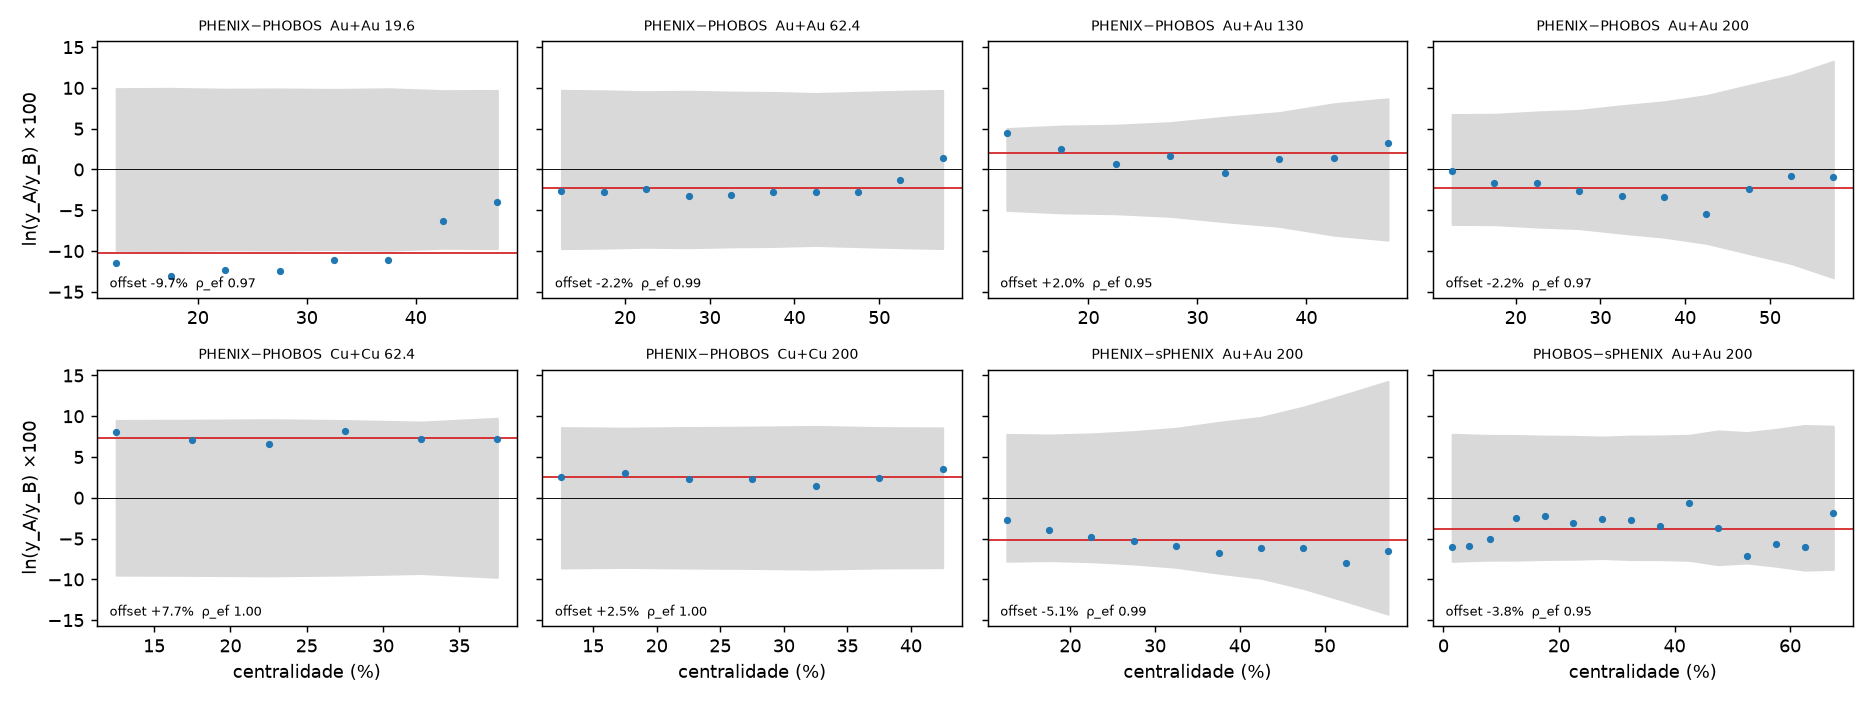
\includegraphics[width=0.92\linewidth]{img/razoes_por_conjunto.png}
\caption{$\ln(y_A/y_B)$ por classe de centralidade. Faixa cinza: incerteza citada. Os pontos formam curvas suaves, muito mais estreitas que
a faixa: o erro é quase todo correlacionado entre classes.}
\end{figure}
\begin{center}\small
\begin{tabularx}{\linewidth}{@{}l Y@{}}
\toprule
momento & resultado \\
\midrule
2º (correlação) & \textbf{medido}. $\rho_{\rm ef}=0{,}95$--$1{,}00$ entre classes. A covariância tem posto $\approx2$: um offset comum (CS com $\rho\approx1$)
mais uma inclinação em centralidade, além de 0,5--2\% diagonal. Isso dá apoio empírico ao CS do degrau 1. \\
2º (tamanho) & Os offsets ficam dentro das incertezas citadas (pull rms $\approx0{,}7$): as incertezas publicadas são, se algo, conservadoras. \\
3º (assimetria) & Assimetria dos resíduos padronizados: $\mathbf{-0{,}08\pm0{,}24}$ (74 resíduos, bootstrap). Dos offsets: $+0{,}13$ com $N=8$.
\textbf{Compatível com zero.} \\
\bottomrule
\end{tabularx}
\end{center}

\subsection{R1 --- parte ímpar do PHOBOS (simetria east/west)}
Usamos as 11 classes de centralidade e 27 pares $\pm\eta$ dos arquivos da calibração.
\begin{figure}[H]
\centering
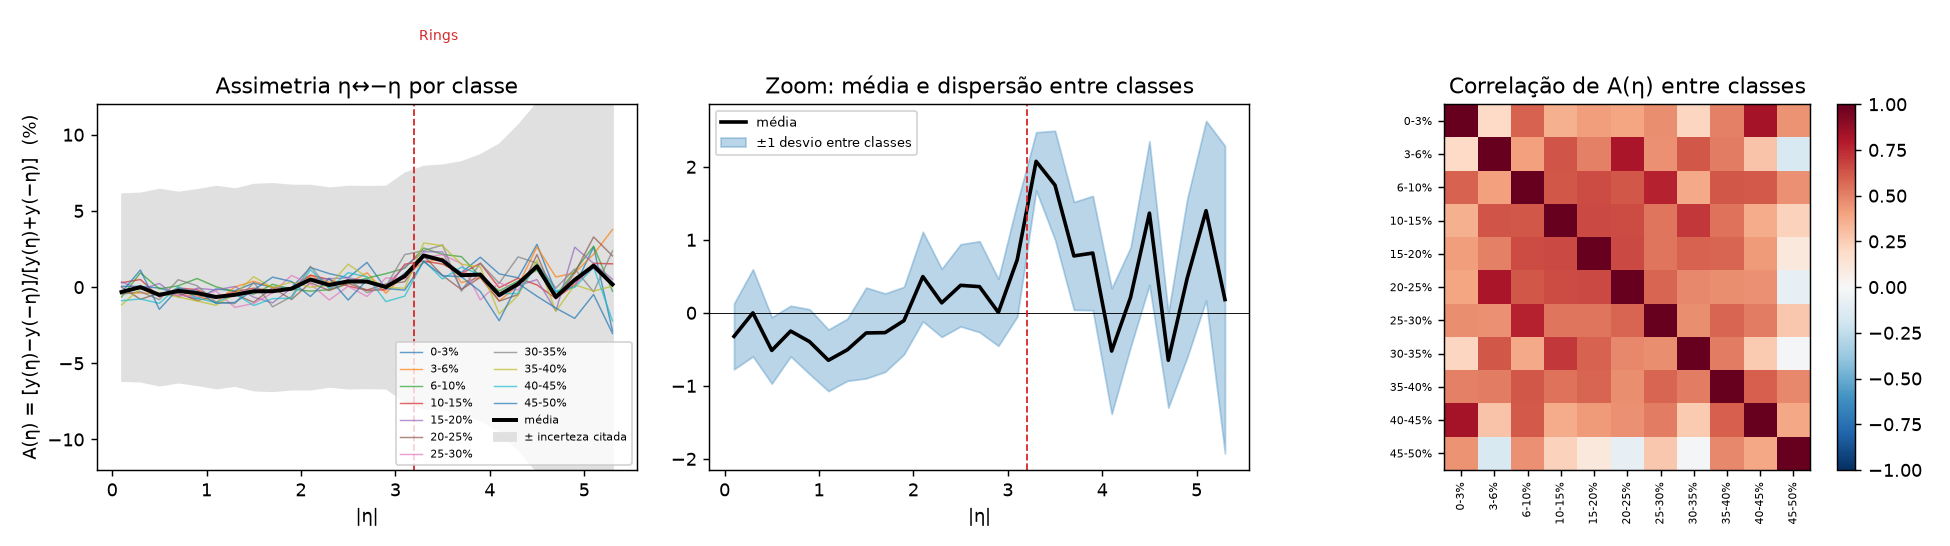
\includegraphics[width=0.92\linewidth]{img/R1_simetria.png}
\caption{$A(\eta)$ por classe; média e dispersão entre classes; correlação entre classes. A linha vermelha marca a fronteira Octagon/Rings.}
\end{figure}
\begin{itemize}[nosep]
\item \textbf{Forma medida a partir dos dados:} um degrau de $\approx2\%$ na fronteira Octagon/Rings e um padrão alternado de $\pm1{,}5\%$ nos Rings,
comuns a todas as classes. O 1º modo da SVD explica 53\% da variância.
\item \textbf{Tamanho:} 10--14\% da incerteza citada (0,7\% no Octagon, 1,5\% nos Rings).
\item \textbf{3º momento: não mensurável.} Só há \emph{uma} realização da fonte (uma análise do PHOBOS), vista em muitos $\eta$.
A assimetria de $A$ descreve o perfil em $\eta$, não a distribuição de probabilidade.
\end{itemize}

\subsection{Por que o 3º momento não foi medido}
\begin{enumerate}[nosep]
\item \textbf{Poucas realizações.} A normalização é comum a todas as classes de um conjunto: $N_{\rm ef}\approx7$. Em réplicas sintéticas,
o Tensor PCA precisa de $N\gtrsim3000$ (seção~\ref{sec:toy}). Faltam cerca de 3 ordens de grandeza.
\item \textbf{Só a assimetria relativa.} $\kappa_3(A-B)=\kappa_3(A)-\kappa_3(B)$, e com três detectores as diferenças somam zero. A variância
de cada detector se separa (three-cornered hat); a assimetria absoluta não, sem uma âncora.
\item \textbf{Os métodos mudam entre runs.} Diferenças de método (não-fluxo, $v\{2\}$ contra $v\{4\}$) se misturam ao sistemático instrumental.
\end{enumerate}
\caixa{orange!10}{\textbf{Leitura.} O que os dados públicos permitem aprender é o \emph{segundo} momento. O terceiro exige réplicas que só a colaboração
tem: variações de cortes, de calibração, de método. \textbf{Pedido aos experimentos:} publicar as variações sistemáticas, e não só as barras de erro.}

\textbf{Ponto em aberto encontrado na 2a:} no arquivo da calibração, a incerteza do PHOBOS em $\eta\approx0$ (6--7,5\%) é compatível com o valor
em 90\% C.L., e não com $1\sigma$ ($\sim$4,6\%). O JETSCAPE pode ter inflado esses sistemáticos em cerca de $1{,}6\times$. É preciso confirmar.

% =====================================================================
\section{Validação em réplicas sintéticas e efeito na posterior}\label{sec:toy}
Como não há réplicas reais, testamos a cadeia completa num toy no binning \emph{real} do STAR $v_2\{2\}(\eta)$ 20--70\% (21 bins, TPC e FTPC).
\begin{itemize}[nosep]
\item \textbf{Fontes postuladas} (formas e tamanhos escolhidos dentro do orçamento de erro publicado; não são a decomposição do STAR):
  \begin{itemize}[nosep]
  \item normalização de 5\%;
  \item assimetria FTPC frente/trás;
  \item borda da FTPC;
  \item na variante 02\_11, a normalização é separada para TPC e FTPC.
  \end{itemize}
\item \textbf{Amplitudes:} Gamma com assimetria 2,0, 1,5 e 2,5.
\item \textbf{Réplicas:} 5000.
\item \textbf{Recuperação:} Tensor PCA, ou seja, CP simétrica de $\hat\kappa_3$ (power iteration, deflação e mínimos quadrados).
\end{itemize}
\begin{figure}[H]
\centering
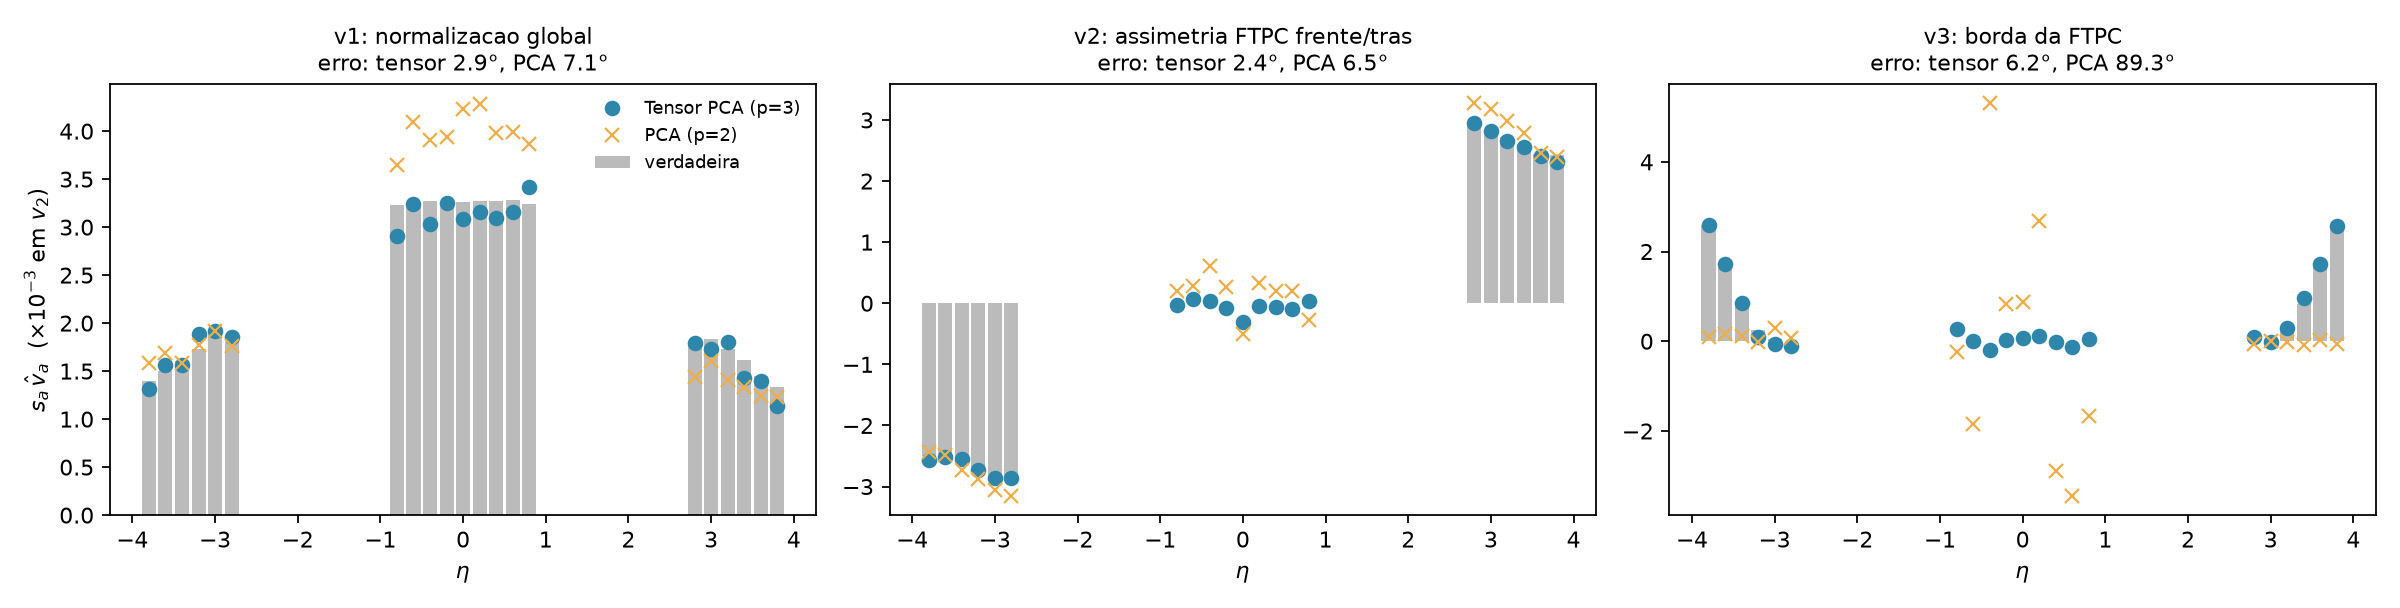
\includegraphics[width=0.66\linewidth]{img/sources_true_vs_recovered.png}\hfill
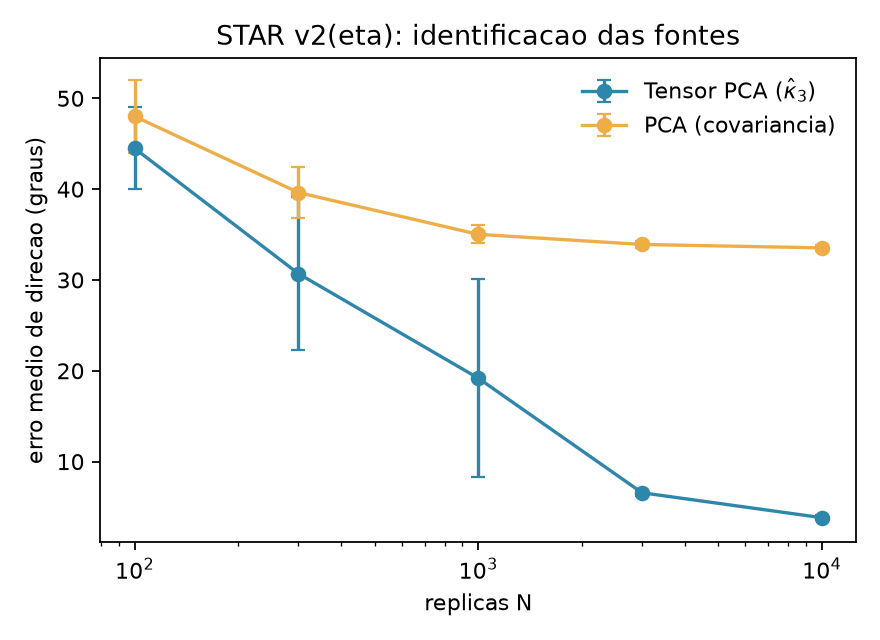
\includegraphics[width=0.32\linewidth]{img/sources_recovery_vs_N.png}
\caption{Esquerda: fontes verdadeiras contra as recuperadas. Direita: erro de direção contra o número de réplicas $N$ (Tensor PCA contra PCA da covariância).}
\end{figure}
\begin{center}\small
\begin{tabular}{@{}lcccc@{}}
\toprule
fonte (02\_11) & skew verdadeiro & skew recuperado & erro dir., Tensor PCA & erro dir., PCA ($p=2$) \\
\midrule
normalização TPC & 2,0 & 1,94 & 3,0° & 2,4° \\
normalização FTPC & 2,0 & 1,91 & 6,4° & \textbf{80,5°} \\
assimetria FTPC & 1,5 & 1,42 & 3,8° & 6,3° \\
borda FTPC & 2,5 & 2,36 & 10,5° & \textbf{89,6°} \\
\bottomrule
\end{tabular}
\end{center}
O erro de direção do Tensor PCA cai de 44° ($N=100$) para 3,8° ($N=10^4$). A PCA da covariância estaciona em cerca de 34°, pela ambiguidade de rotação.

\textbf{Efeito na posterior.} As fontes recuperadas entram como nuisances $\lambda_a$ (prior Gamma) amostradas junto com $\theta$.
São as cadeias 02\_10 e 02\_11: 23 e 24 parâmetros, $200\times20\,000$ passos.
\begin{figure}[H]
\centering
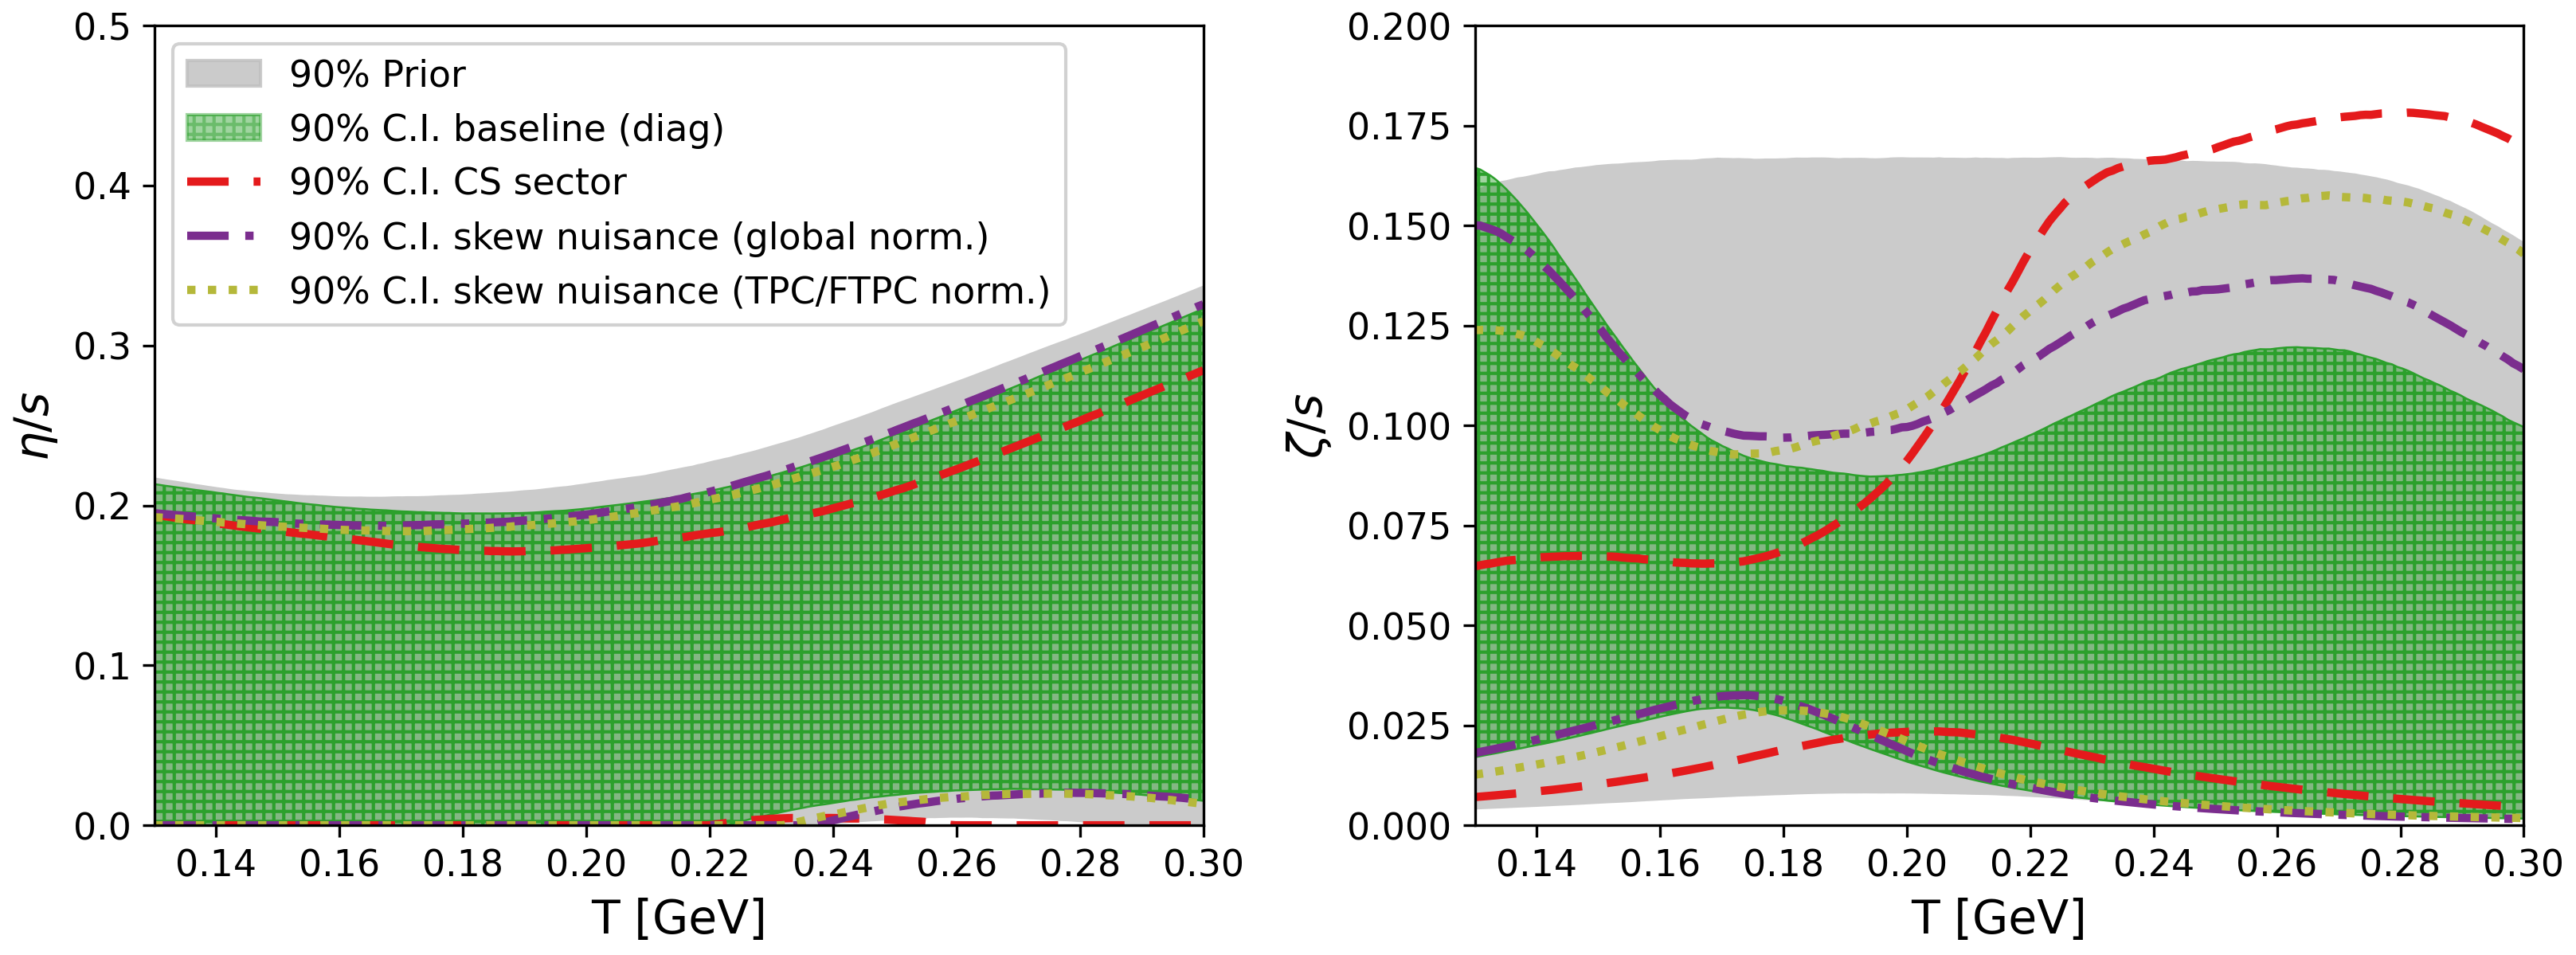
\includegraphics[width=0.49\linewidth]{img/F14-viscosity__covmom__baseline-cs-nuisglob-nuissplit.png}\hfill
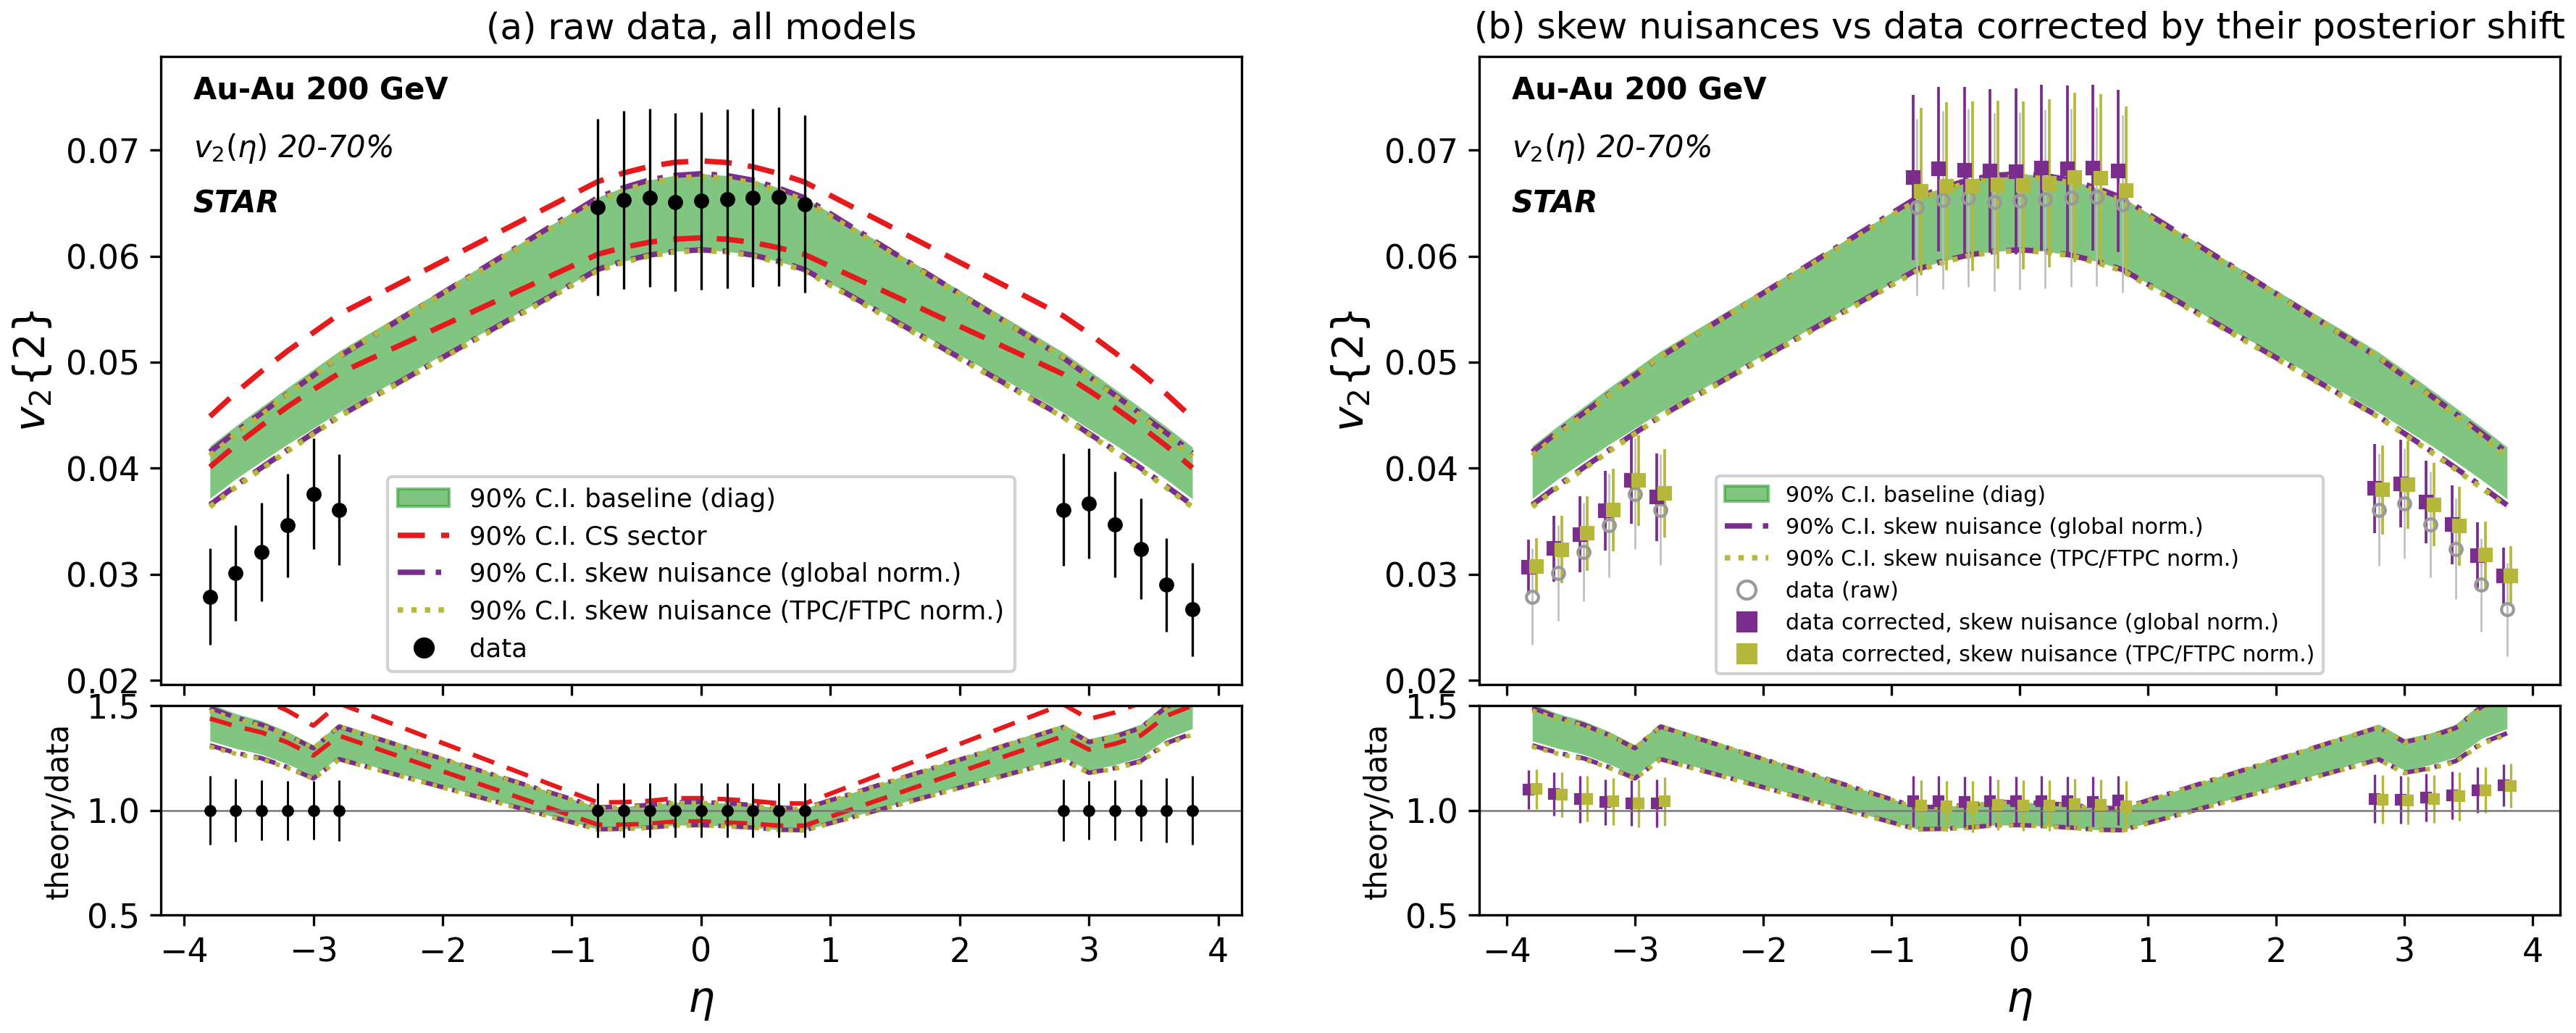
\includegraphics[width=0.49\linewidth]{img/F05-observables__covmom__baseline-cs-nuisglob-nuissplit__star-v2eta-20-70.png}
\caption{Esquerda: $\eta/s(T)$ e $\zeta/s(T)$. Direita: STAR $v_2(\eta)$ 20--70\%; em (b), os dados corrigidos pelo deslocamento posterior $\sum_a\lambda_a\vhat_a$.}
\end{figure}
\begin{itemize}[nosep]
\item Com uma assimetria plausível, a posterior de $\theta$ \textbf{quase não muda}, bem menos que com o CS sector.
\item A tensão na FTPC (modelo cerca de 30\% acima) \textbf{não} é explicada por sistemáticos assimétricos do tamanho publicado: $\lambda$
fica presa na borda do suporte da Gamma. A tensão é do modelo, não do erro.
\end{itemize}

% =====================================================================
\section{O \emph{case} para computação quântica}
\subsection{O problema computacional}
Dadas $N$ réplicas $y^{(r)}\in\mathbb R^n$ de um bloco de detector, estimar
\[
\hat\kappa_3=\tfrac1N\sum_r (y^{(r)}-\bar y)^{\otimes3}=\sum_a w_a\,\vhat_a^{\otimes3}+G,
\]
e recuperar $\{\vhat_a,w_a\}$. Com uma fonte, é o \textbf{spiked tensor model} de ordem $p=3$, $Y=\beta x^{\otimes3}+G$.
Com várias, é a decomposição CP simétrica.

\subsection{Algoritmo e ganho esperado}
\begin{center}\small
\begin{tabularx}{\linewidth}{@{}l Y@{}}
\toprule
Algoritmo & Tensor PCA quântico de Hastings (spectral method de Kikuchi, nível $\ell$, com estimação de fase).
Classificado como ganho \textbf{super-quadrático} (quártico) em Kammerlander, O'Brien, King \emph{et al.}, arXiv:2610.32595 (2026), Sec.~4.1. \\
Custo clássico & $\sim n^{\ell}$ \\
Custo quântico & $\sim n^{\ell/4}\,\mathrm{poly}(n)$; memória $O(\ell\log n)$ qubits \\
Regime útil & janela ``difícil, mas detectável'': $n^{-p/4}\gtrsim\beta\gg n^{(1-p)/2}$, isto é, fontes fracas e $n$ grande \\
Onde \textbf{não} há ganho & covariância ($p=2$): a PCA matricial já é eficiente (os próprios autores excluem). Sistemas lineares
$\Sigma^{-1}r$ com $n\sim10^3$: Cholesky é trivial. O ganho está no \textbf{3º momento}. \\
\bottomrule
\end{tabularx}
\end{center}

\subsection{O que já foi feito (demonstração de correção, não de vantagem)}
\arq{study_nongaussian_systematics/quantum/quantum_tensor_pca.py}: Tensor PCA com o passo espectral feito por \textbf{QPE em Qiskit Aer}.
\begin{itemize}[nosep]
\item O passo espectral é o autovetor dominante de $M(u)=\kappa_3(\cdot,\cdot,u)$.
\item 21 bins preenchidos até 32, ou seja 5 qubits de sistema; mais 9 de relógio; \textbf{14 qubits} no total.
\end{itemize}
\begin{figure}[H]
\centering
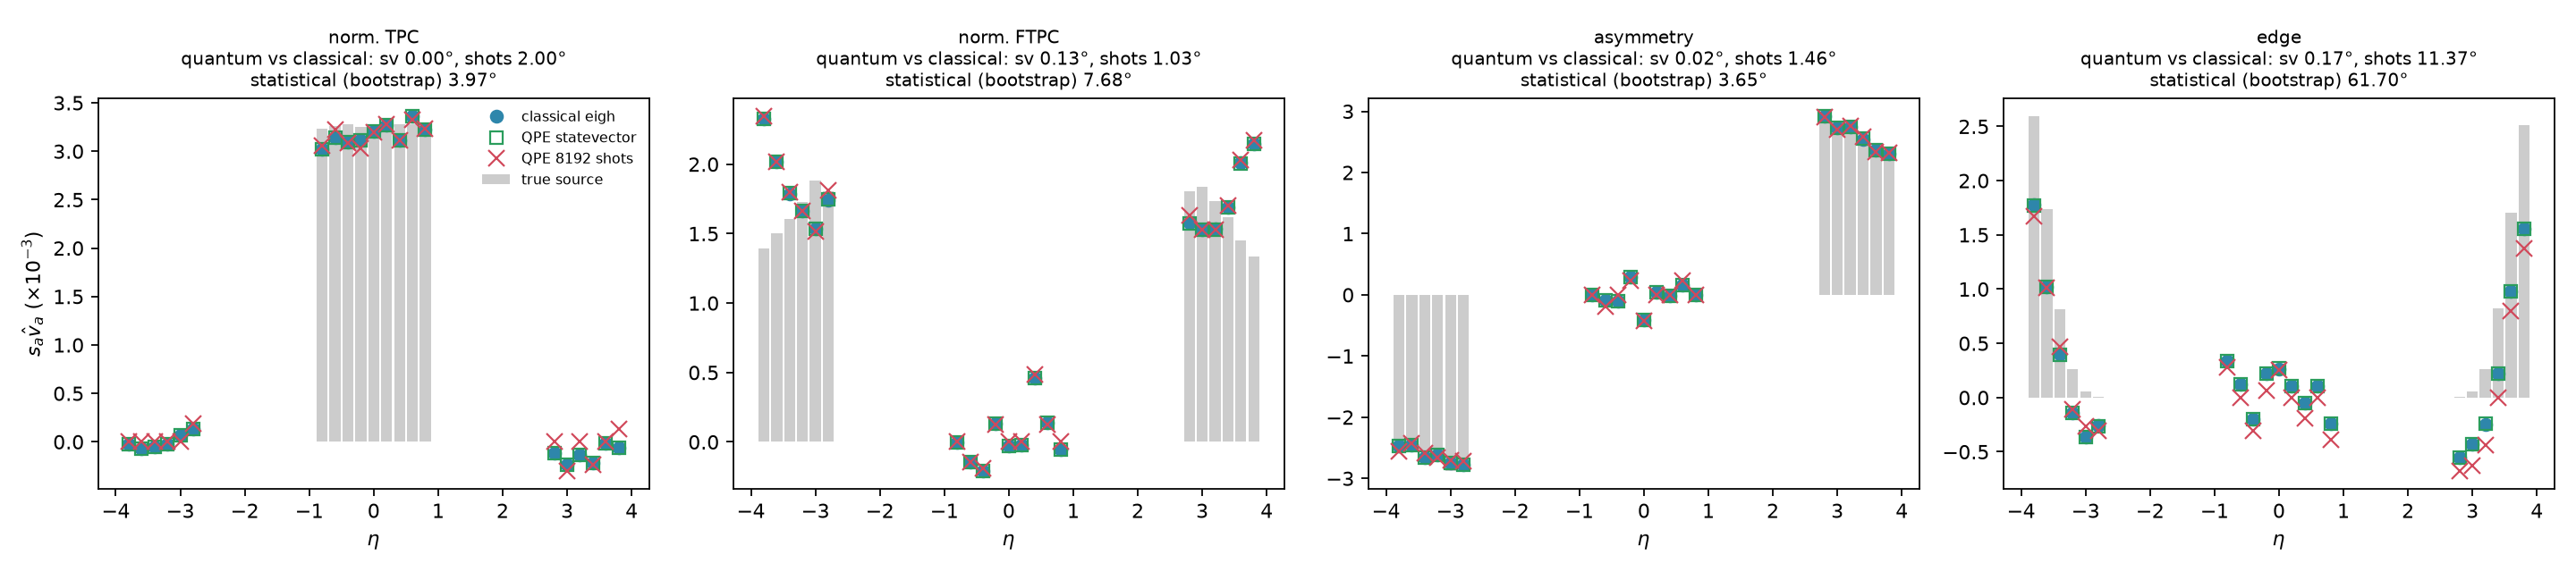
\includegraphics[width=0.75\linewidth]{img/quantum_vs_classical_sources.png}
\caption{Fontes recuperadas: clássico ($\mathtt{eigh}$), QPE com statevector e QPE com 8192 shots (5000 réplicas, 02\_11).}
\end{figure}
\begin{center}\small
\begin{tabular}{@{}lccc@{}}
\toprule
& clássico & QPE statevector & QPE shots \\
\midrule
tempo & 3 s & 33 s (288 circuitos) & 347 s (10\,703 circuitos) \\
ângulo até o clássico, bruto & --- & $\le0{,}17°$ & 1--11° (pior na borda) \\
ângulo até o clássico, após refinamento & --- & 0,0° & 0,0° \\
\bottomrule
\end{tabular}
\end{center}

\subsection{Recursos para os tamanhos reais}
\begin{center}\small
\begin{tabular}{@{}lccc@{}}
\toprule
bloco & $n$ & $\log_2 n$ & qubits $\sim\ell\log_2 n$ \\
\midrule
STAR $v_2(\eta)$ (21 bins) & 21 & 4,4 & $4{,}4\,\ell$ \\
PHOBOS $dN/d\eta$ (maior bloco de hardware) & 594 & 9,2 & $9{,}2\,\ell$ \\
toda a calibração & 917 & 9,8 & $9{,}8\,\ell$ \\
\bottomrule
\end{tabular}
\end{center}
O tamanho relevante é o do maior bloco de um mesmo detector, não 917, porque fontes de detectores diferentes são independentes.
Nesses tamanhos, a CP clássica leva segundos. O ganho aparece em análises globais ($n\gg10^3$, muitos observáveis e experimentos),
em fontes fracas (dentro da janela difícil) e em ordem mais alta ($p=4$, caudas).

\subsection{O que levar para a escola}
\begin{enumerate}[nosep]
\item \textbf{Um problema físico real que é um spiked tensor.} As fontes sistemáticas assimétricas de um detector são autovetores de $\kappa_3$.
A covariância não as identifica: a PCA erra a direção em 80--90°.
\item \textbf{A tentativa com dados reais mostra onde está o gargalo.} Há no máximo 1--3 runs independentes por medida e $N_{\rm ef}\approx7$
nas comparações entre detectores, contra $N\gtrsim3000$ necessárias. O 2º momento sai (CS $\rho\approx1$ confirmado); o 3º não.
\item \textbf{Um critério de precisão vindo da física.} A posterior quase não reage ao valor exato do skew. O solver precisa acertar direções e ordem
de grandeza, não muitos dígitos. Isso favorece algoritmos aproximados e com ruído.
\item \textbf{Honestidade sobre a vantagem.} Com $n=21$--$917$ não há vantagem prática; o QPE no simulador é uma prova de correção.
O caminho de escala depende de os experimentos publicarem réplicas ($\gtrsim10^3$ variações por medida).
\end{enumerate}

% =====================================================================
\section{Próximos passos}
\begin{itemize}[nosep]
\item \textbf{Degrau 3 com o 2º momento aprendido.} Cadeia com a covariância do PHOBOS medida na 2a (offset e inclinação), no lugar da suposta.
É gaussiana, tem o custo de uma cadeia CS, e seria a primeira posterior com estrutura de erro inferida de dados.
\item Confirmar se os sistemáticos do PHOBOS (90\% C.L.) foram usados como $1\sigma$ na calibração.
\item Fatias 2b e 2c (forma em $\eta$: PHOBOS--sPHENIX, PHOBOS--BRAHMS), R2 (simetria do STAR $v_2(\eta)$) e 2d ($v_2(p_T)$ STAR--PHENIX).
\item Contato com as colaborações para obter variações sistemáticas reais.
\end{itemize}

\section*{Arquivos}
\small
\begin{itemize}[nosep]
\item Levantamento e fatias (cópia local, ainda não sincronizada com o HPC):
  \begin{itemize}[nosep]
  \item pasta: \arq{IFUSP-Heavy-Ions/3dglauber-bayes-exemple/3dglauber-bayes-example/study_nongaussian_systematics/};
  \item arquivos: \arq{MAPA.tex}, \arq{replicas_survey.md}, \arq{cross_detector_overlaps.md}, \arq{fatia2a/}, \arq{regiao_eta/}, \arq{data/}.
  \end{itemize}
\item Toy, Tensor PCA e QPE (HPC): \arq{3dglauber-bayes-example/study_nongaussian_systematics/\{toy_model,quantum\}/}.
\item Cadeias: \arq{mcmc/02_10_nongaussian_nuisance/}, \arq{mcmc/02_11_nongaussian_nuisance_detector_split/}.
\item Proveniência das fontes do toy: \arq{../INFERENCE.md}.
\end{itemize}
\end{document}
